%%%%%%%%%%%%%%%%%%%%%%%%%%%%%%%%%%%%%%%%%%%%%%%%
\subsection{Strange hadron abundance in cosmic plasma}
\label{Strangeness}\index{strangeness}
%%%%%%%%%%%%%%%%%%%%%%%%%%%%%%%%%%
\para{Hadron populations in equilibrium}
As the Universe expanded and cooled down to the QGP Hagedorn temperature\index{Hagedorn!temperature} $T_H\approx150\MeV$, the primordial QGP underwent a phase transformation called hadronization. Quarks and gluons fragmented, combined and formed matter and antimatter we are familiar with. After hadronization\index{hadrons!hadronization}, one may think that all relatively short lived massive hadrons decay rapidly and disappear from the Universe. However, the most abundant hadrons\index{hadrons}, pions $\pi(q\bar q)$, can be produced via their inverse decay process $\gamma\gamma\rightarrow\pi^0$. Therefore they retain their chemical equilibrium down to $T=3\sim5\MeV$~\cite{Kuznetsova:2008jt}. 

{\color{black} This result demonstrates a key difference between laboratory heavy-ion experiments and the the hot hadronic Universe: In the evolving Universe we allow for a full adjustment in the particle inventory to the ambient temperature, and we follow this inventory as a function of temperature with chemical potential(s) constrained by the baryon asymmetry, this is how the overview \rf{fig:energy:frac} was obtained. The key dynamic difference between Universe and laboratory is that in the former each particle has individual decoupling conditions while in the letter we study only strongly interacting particles, which all freeze-out near to phase cross-over from QGP to the hadron phase: Laboratory experimental data provide snap-shot image of QGP explosion into hadrons. For our study of laboratory environment see Ref.\,\cite{Letessier:2005qe,Petran:2013qla,Rafelski:2014cqa}. It is the mastery of the methods developed in the study of relativistic heavy-ion collisions that makes precise modeling of the primordial Universe possible.}

We begin by determining the Universe particle population composition assuming both kinetic and particle abundance equilibrium (chemical equilibrium) of non-interacting bosons and fermions. By considering the charge neutrality\index{charge neutrality} and a prescribed conserved baryon-per-entropy-ratio\index{baryon!entropy ratio} ${(n_B-n_{\overline{B}})}/{\sigma}$ we can determine the baryon chemical potential\index{chemical potential!baryon} $\mu_B$~\cite{Fromerth:2002wb,Fromerth:2012fe,Rafelski:2013yka}. We extend this approach allowing for the presence of strange hadrons, and imposing conservation of strangeness in the primordial Universe -- the strange quark content in hadrons must equal the anti-strange quark content in statistical average $\langle s-\bar s \rangle=0$. 

Given $\mu_B(T)$, $\mu_s(T)$ the baryon and strangeness chemical potentials as a function of temperature, we can obtain the particle number densities for different strange and non-strange species and study their population in the primordial Universe. Our approach prioritizes strangeness pair production into bound hadron states by either strong or electromagnetic interactions, or both, over the also possible weak interaction strangeness changing processes, which are capable to amplify the effect of baryon asymmetry. This is another topic beyond the scope of this work deserving further attention.

To characterize the baryon and strangeness content of a hadron we employ the chemical fugacity\index{fugacity!strangeness} for strangeness $\lambda_s$ and for light quarks $\lambda_q$ \index{quark!fugacity}
\begin{align}
\lambda_s=\exp(\mu_s/T)\,\quad \lambda_q=\exp(\mu_B/3T)\,.
\end{align}
Here $\mu_s$ and $\mu_B$ are the chemical potential of strangeness and baryon, respectively. To obtain quark fugacity\index{fugacity!quark} $\lambda_q$, we divide the baryo-chemical potential of baryons by quark content in the baryon, \ie\ three.

When the baryon chemical potential does not vanish, the chemical potential of strangeness in the primordial Universe is obtained by imposing the conservation of strangeness constraint $\langle s-\bar s \rangle=0$, see Section 11.5 in Ref.\,\cite{Letessier:2002ony}\index{strangeness! chemical potential} which leads considering only the dominant single strange hadrons to the condition
\begin{align}\label{museq}
\lambda_s=\lambda_q\sqrt{\frac{F_K+\lambda^{-3}_q\,F_Y}{F_K+\lambda^3_q\,F_Y}}\,.
\end{align}
Here we employ the phase-space function $F_i$ for sets of nucleon $N$, kaons $K$, and hyperon\index{hyperon} $Y$ particles 
\begin{align}
&F_N=\sum_{N_i}\,g_{N_i}W(m_{N_i}/T)\;, \quad N_i=n, p, \Delta(1232),\\
&F_K=\sum_{K_i}\,g_{K_i}W(m_{K_i}/T)\;, \quad K_i=K^0, \overline{K^0}, K^\pm, K^\ast(892),\\
&F_Y=\sum_{Y_i}\,g_{Y_i}W(m_{Y_i}/T)\;, \quad Y_i=\Lambda, \Sigma^0,\Sigma^\pm, \Sigma(1385),
\end{align}
$g_{N_i,K_i,Y_i}$ are the degeneracy factors, and the function $W(x)=x^2K_2(x)$ was introduced in \req{DensityH}.

Considering the massive particle number density in the Boltzmann\index{Boltzmann!approximation} approximation, we obtain
\begin{align}
\label{Density_N}
&n_N=\frac{T^3}{2\pi^2}\lambda_q^3F_N,\quad\qquad\qquad n_{\overline N}=\frac{T^3}{2\pi^2}\lambda^{-3}_qF_N,\\
\label{Density_K}
&n_K=\frac{T^3}{2\pi^2}\left(\lambda_s\lambda_q^{-1}\right)F_K,\,\qquad n_{\overline{K}}=\frac{T^3}{2\pi^2}\left(\lambda_s^{-1}\lambda_q\right)F_K,\\
\label{Density_Y}
&n_Y=\frac{T^3}{2\pi^2}\left(\lambda_q^2\lambda_s\right)F_Y,\quad\qquad n_{\overline Y}=\frac{T^3}{2\pi^2}\left(\lambda^{-2}_q\lambda_s^{-1}\right)F_Y.
\end{align}
In this case, the net baryon density in the primordial Universe with temperature range $150\MeV> T>10\MeV$ can be written as 
\begin{align}
\frac{\left(n_B-n_{\overline{B}}\right)}{\sigma}&=\frac{1}{\sigma}\left[\left(n_p-n_{\overline{p}}\right)+\left(n_n-n_{\overline{n}}\right)+\left(n_Y-n_{\overline{Y}}\right)\right]\notag\\
&=\frac{T^3}{2\pi^2\,\sigma}\left[\left(\lambda_q^3-\lambda^{-3}_q\right)F_N+\left(\lambda_q^2\lambda_s-\lambda^{-2}_q\lambda_s^{-1}\right)F_Y\right]\notag\\
&=\frac{T^3}{2\pi^2\sigma}\left(\lambda_q^3-\lambda_q^{-3}\right)F_N\left[1+\frac{\lambda_s}{\lambda_q}\left(\frac{\lambda_q^3-\lambda^{-1}_q\lambda_s^{-2}}{\lambda^3_q-\lambda^{-3}_q}\right)\,\frac{F_Y}{F_N}\right]\notag\\
&\approx\frac{T^3}{2\pi^2\sigma}\left(\lambda_q^3-\lambda_q^{-3}\right)F_N\left[1+\frac{\lambda_s}{\lambda_q}\,\frac{F_Y}{F_N}\right],
\end{align}
where we can neglect the term $F_Y/F_K$ in the expansion of \req{museq} in our temperature range. 

Introducing the strangeness conservation $\langle s-\bar s\rangle=0$ constraint and using the entropy density\index{entropy!density} in the primordial Universe, the explicit relation for baryon to entropy ratio becomes
\begin{align}\label{muBeq}
\frac{n_B-n_{\overline{B}}}{\sigma}&=\frac{45}{2\pi^4g^s_\ast}\sinh\left[\frac{\mu_B}{T}\right]F_N\times\left[1+\frac{F_Y}{F_N}\sqrt{\frac{1+e^{-\mu_B/T}\,F_Y/F_K}{1+e^{\mu_B/T}\,F_Y/F_K}}\right].
\end{align}
The present-day baryon-per-entropy-ratio is needed in \req{muBeq}, see \req{BaryonEntropyRatio}. It is convenient to also remember the quantum value of entropy per particle, for a massless bosons $\sigma/n|_\mathrm{boson}\approx 3.60$, and for a massless fermions $\sigma/n|_\mathrm{fermion}\approx 4.20$. We solve \req{museq}) and \req{muBeq} numerically to obtain baryon and strangeness chemical potentials as functions of temperature shown in the top frame of~\rf{Baryon:fig}.

%%%%%%%%%%%%%%%%%%%%%%%%
\begin{figure}
\centerline{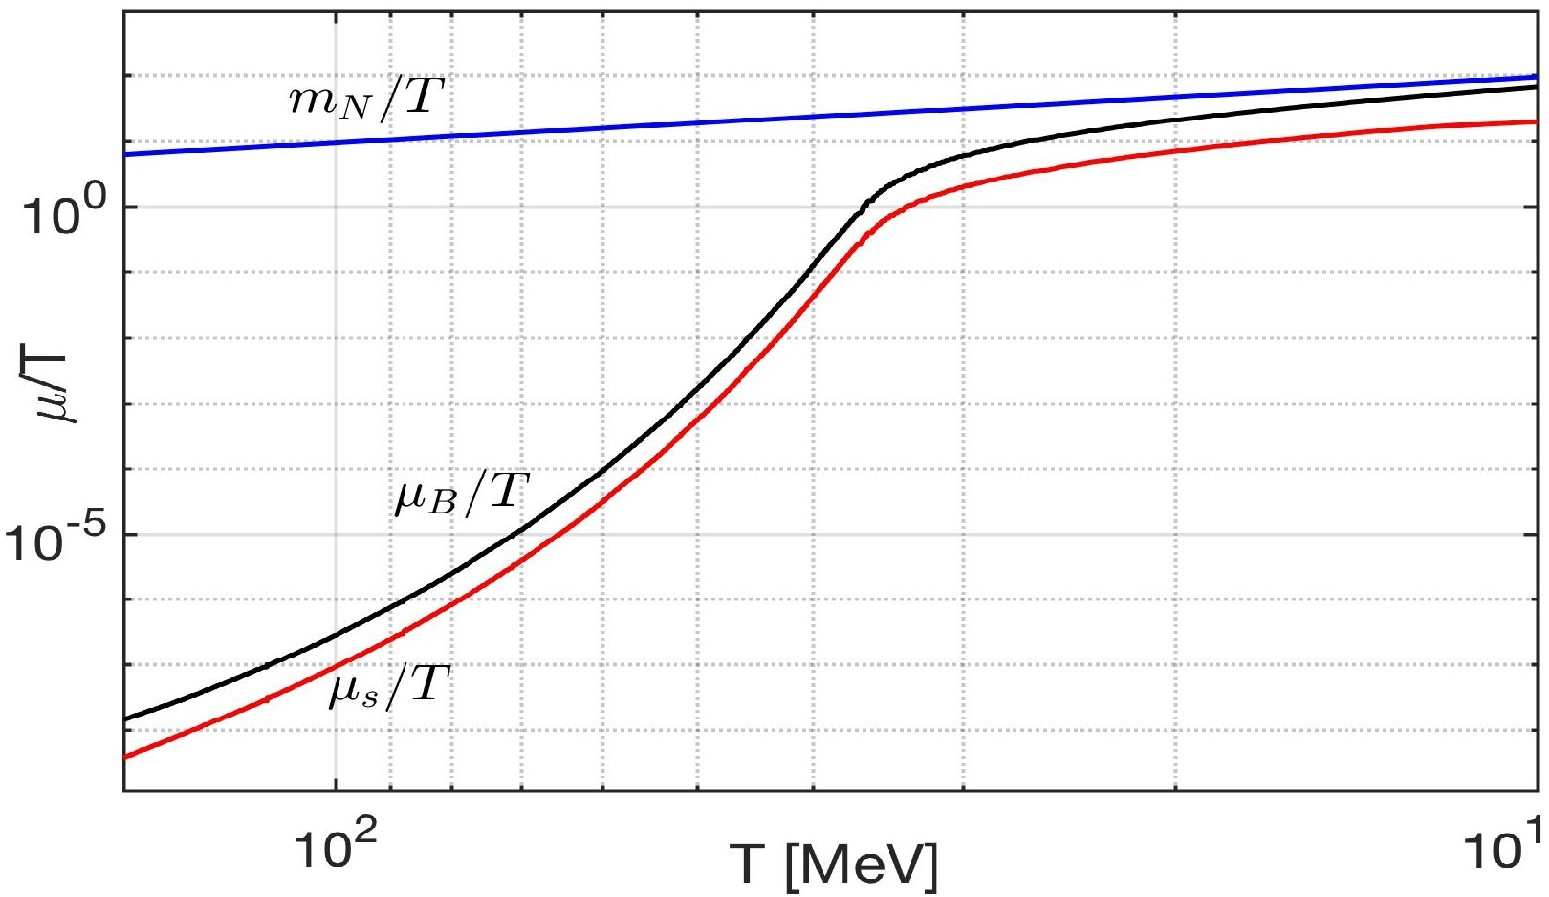
\includegraphics[width=0.82\linewidth]{./plots/New_Chemical_Potential_C.jpg}}
\vspace{-0.55cm}
\centerline{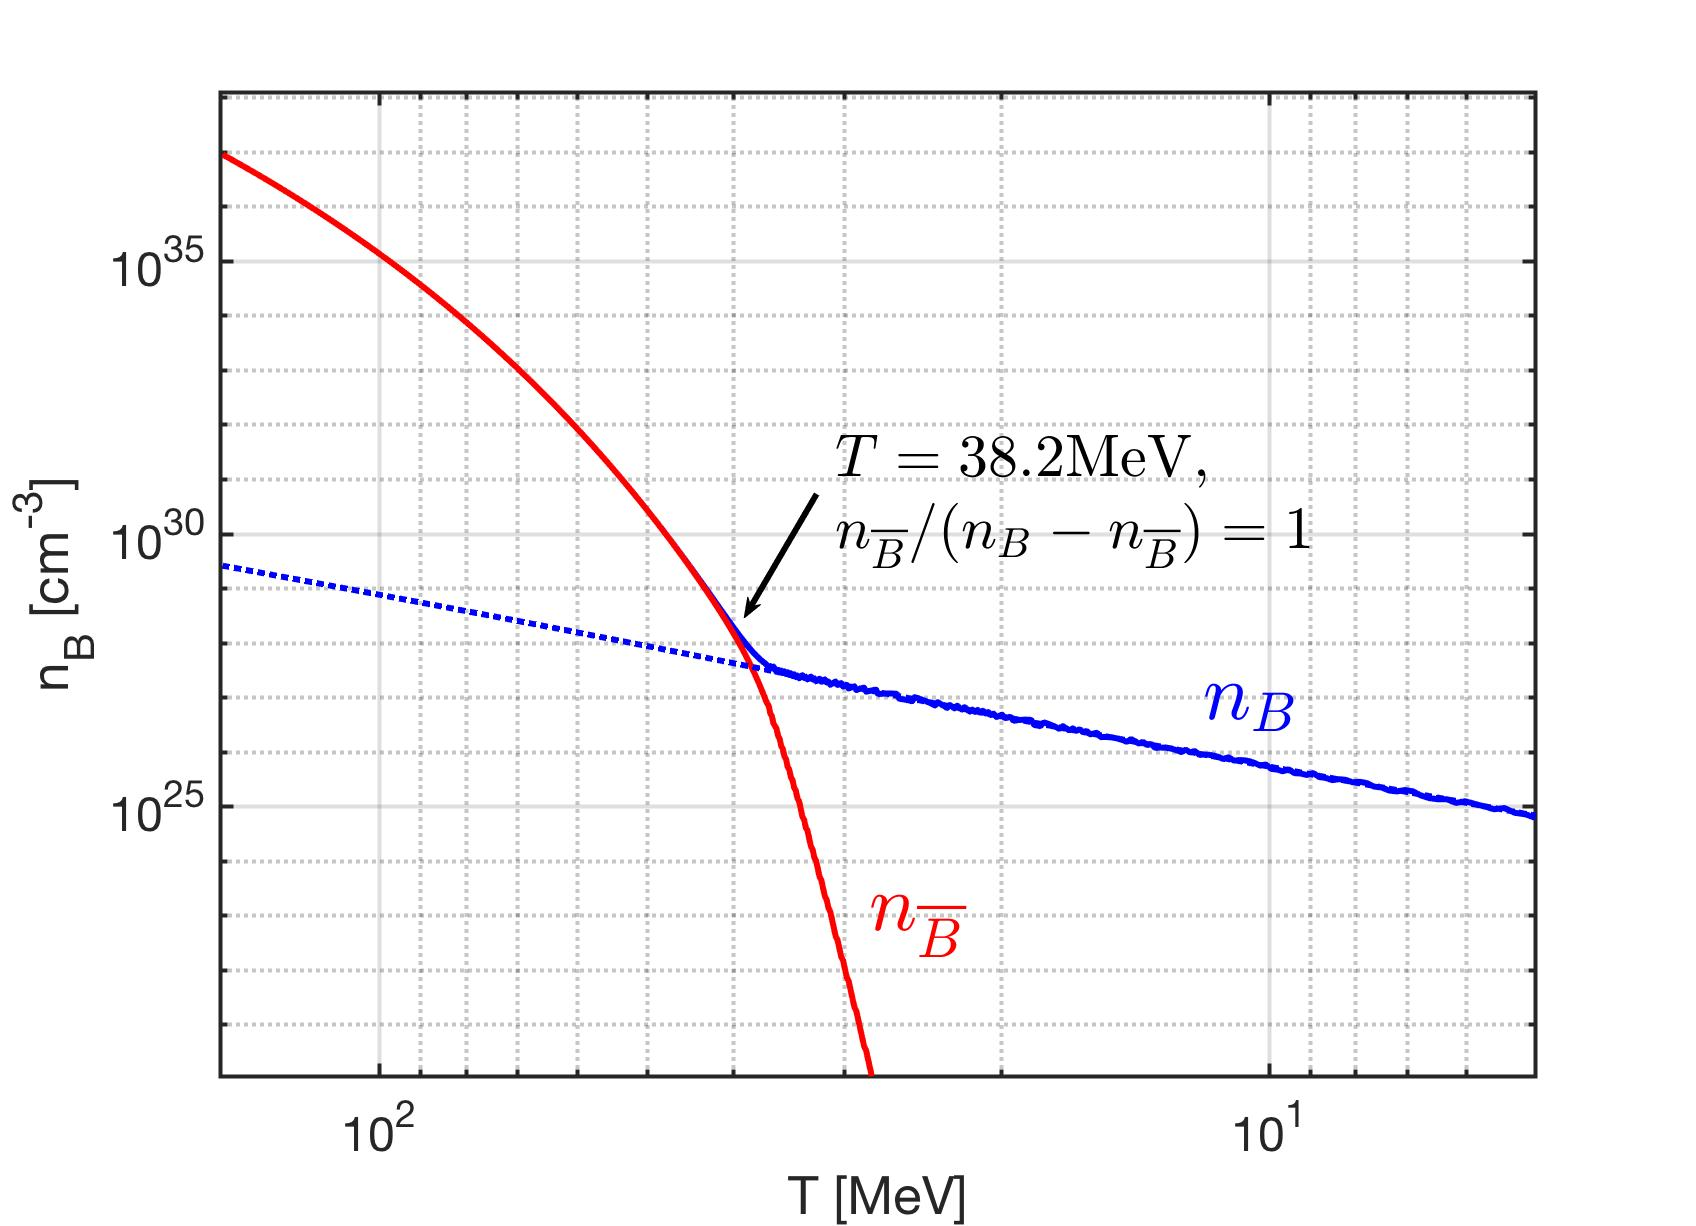
\includegraphics[width=0.84\linewidth]{./plots/Baryon_Antibaryon_cm.jpg}}
\caption{Top frame: Solid (black) line baryon number chemical potential $\mu_B/T$; dotted (red) line strangeness chemical potential $\mu_s/T$, as a function of temperature $150\MeV> T>10\MeV$ in the primordial Universe; for comparison we show dashed (blue) $m_N/T $ with $m_N=938.92\MeV$, the average nucleon mass. \cccite{Yang:2021bko}. \radapt{Yang:2024ret}
\index{strangeness!chemical potential} \index{chemical potential!baryon}
%}
%\label{ChemPotFig} 
%\end{figure}
%%%%%%%%%%%%%%%%%%%%%%%%%%%%%%
%%%%%%%%%%%%%%%%%%%%%%%%%%%%%%%%%%%%%%%
%\begin{figure} 
%\centerline{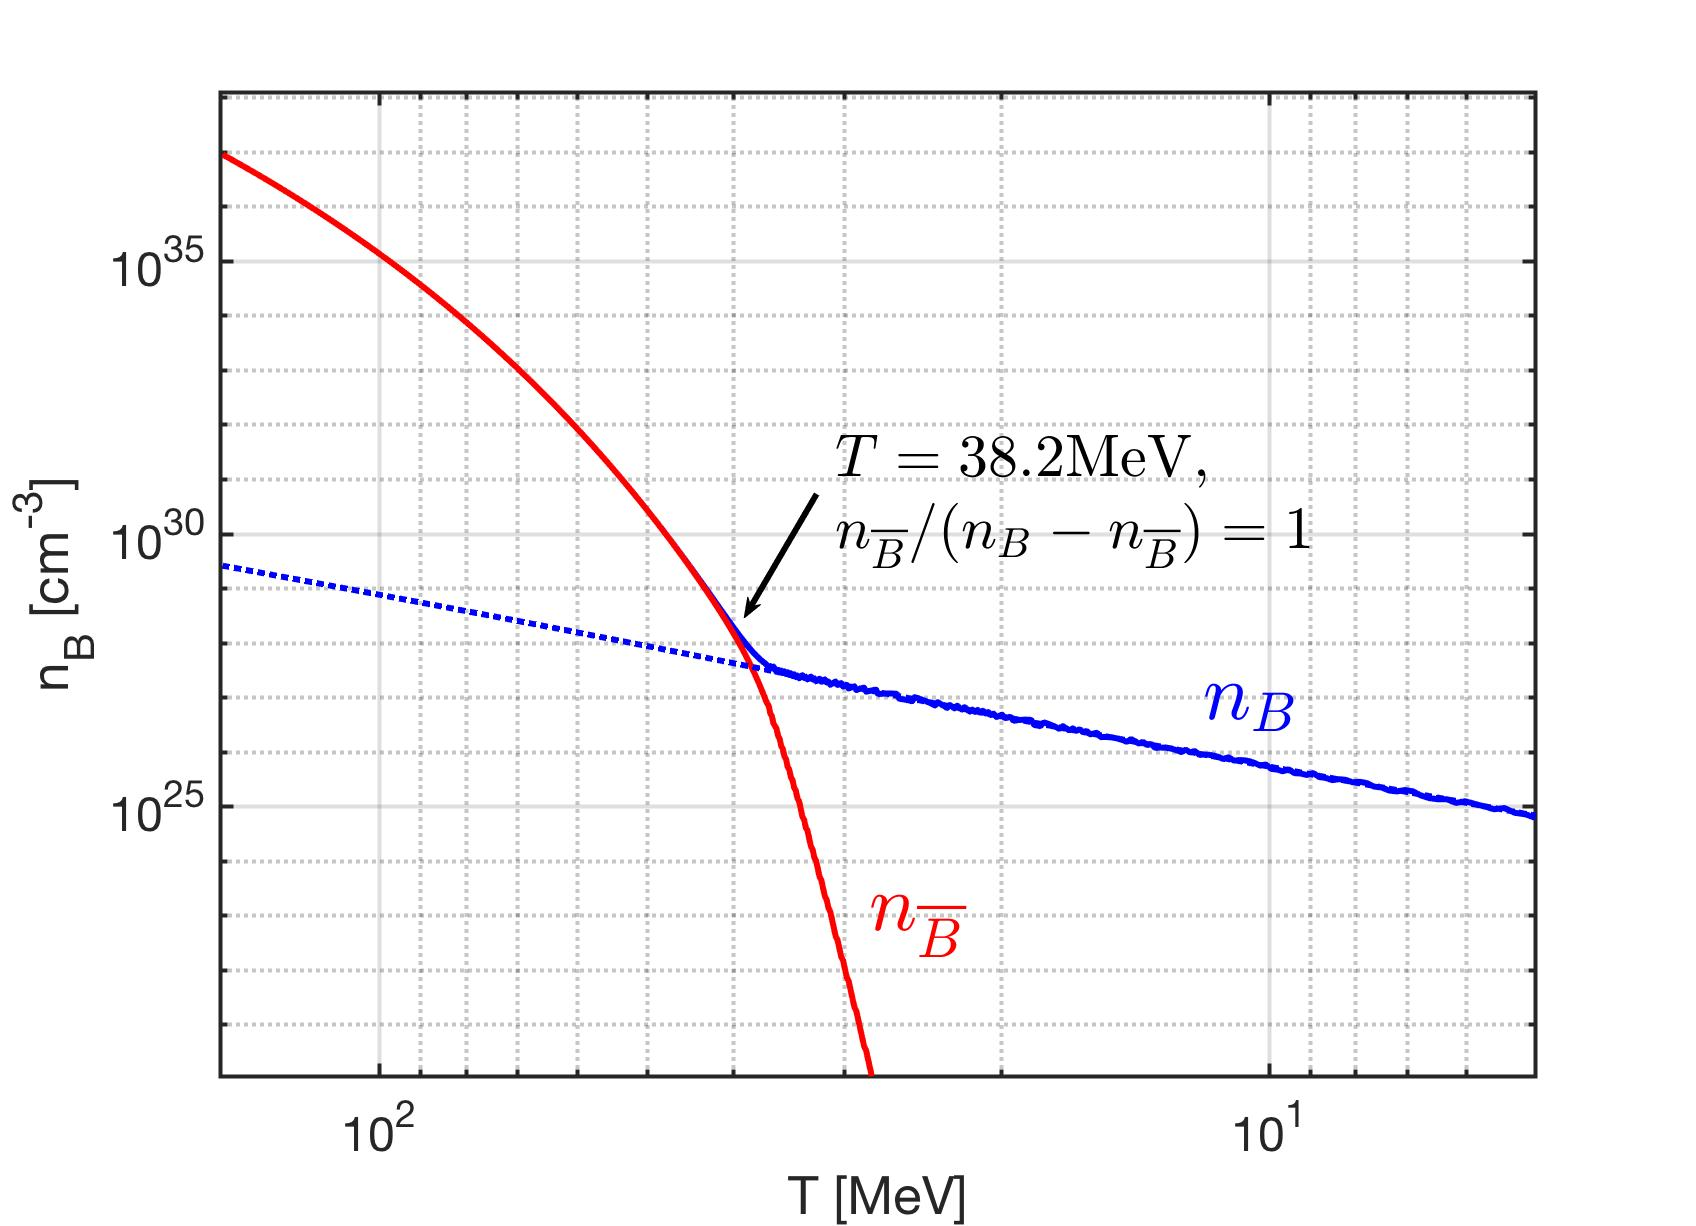
\includegraphics[width=0.85\linewidth]{./plots/Baryon_Antibaryon_cm.jpg}}
%\caption{
{\color{black} Bottom frame: Net baryon number $n_{B}-n_{\overline{B}}$ in temperature range $150\MeV>T>5\MeV$, the dashed (blue) line turns into solid (blue) line depicting baryon density $n_{B}$ once the antibaryon $n_{\overline B}$ number density, solid line (red), diminishes; the transition point $n_{\overline B}/(n_B-n_{\overline B})=1$ is at $T=38.2\MeV$.\index{Antibaryons!in Universe} \cccite{Rafelski:2023emw}. \radapt{Yang:2024ret}}
}
\label{Baryon:fig}
\end{figure}
%%%%%%%%%%%%%%%%%%%%%%%%%%%%%%%%%%%%%%%

The shape of chemical potentials in the top frame of ~\rf{Baryon:fig} changes dramatically, showing a knee in the temperature window $50\MeV\le T\le 30\MeV$. This behavior is describing the antibaryon\index{baryon!antibaryon} disappearance from the Universe inventory. Substituting the chemical potential $\lambda_q$ and $\lambda_s$ into particle density \req{Density_N}, \req{Density_K}, and \req{Density_Y}, we can obtain the particle number densities for different species as functions of temperature. 

The net baryon $n_B-n_{\overline B}$ number density is compared to the antibaryon number density in the bottom frame of~\rf{Baryon:fig}. We note the transition point $n_{\overline B}\ll(n_B-n_{\overline B})=1$ at temperature $T=38.2\MeV$ marking the effective antibaryon disappearance temperature from the Universe inventory. This precisely computed result is in good agreement with the qualitative result presented in 1990 by Kolb and Turner~\cite{Kolb:1990vq}. Below this temperature, antibaryons rapidly disappear, while the baryon density dilutes due to Universe expansion. The baryon to entropy ratio remains constant.

In~\rf{EquilibPartRatiosFig} we present examples of hadronic particle abundance ratios of interest\index{hadrons!abundance ratios}. Pions $\pi(q\bar q)$ are the most abundant hadrons $n_\pi/n_B\gg1$, because of their low mass and the reaction $\gamma\gamma\rightarrow\pi^0$, which assures chemical yield equilibrium~\cite{Kuznetsova:2008jt} in the era of interest here. For $150\MeV>T>20.8\MeV$, we see the ratio $n_{{\overline K}(\bar q s)}/n_B\gg1$, which implies pair abundance of strangeness is more abundant than baryons, and is dominantly present in mesons, since $n_{\overline K}/n_Y\gg1$. This also implies that the exchange reaction $\overline{K}+N\rightarrow \Lambda+\pi$ can re-equilibrate kaons and hyperons; therefore strangeness symmetry $s=\bar s$ can be maintained. Considering $n_Y/n_B$ we see that hyperons\index{hyperon} $Y(sqq)$ remain a noticeable 1\% component in the baryon yield through the domain of antibaryon decoupling. Below $T=12.9\MeV$ we have $n_Y/n_B>n_{\overline K}/n_B$, now the still existent tiny abundance of strangeness is found predominantly in hyperons.

%%%%%%%%%%%%%%%%%%%%%%%%%%%%
\begin{figure} 
\centerline{
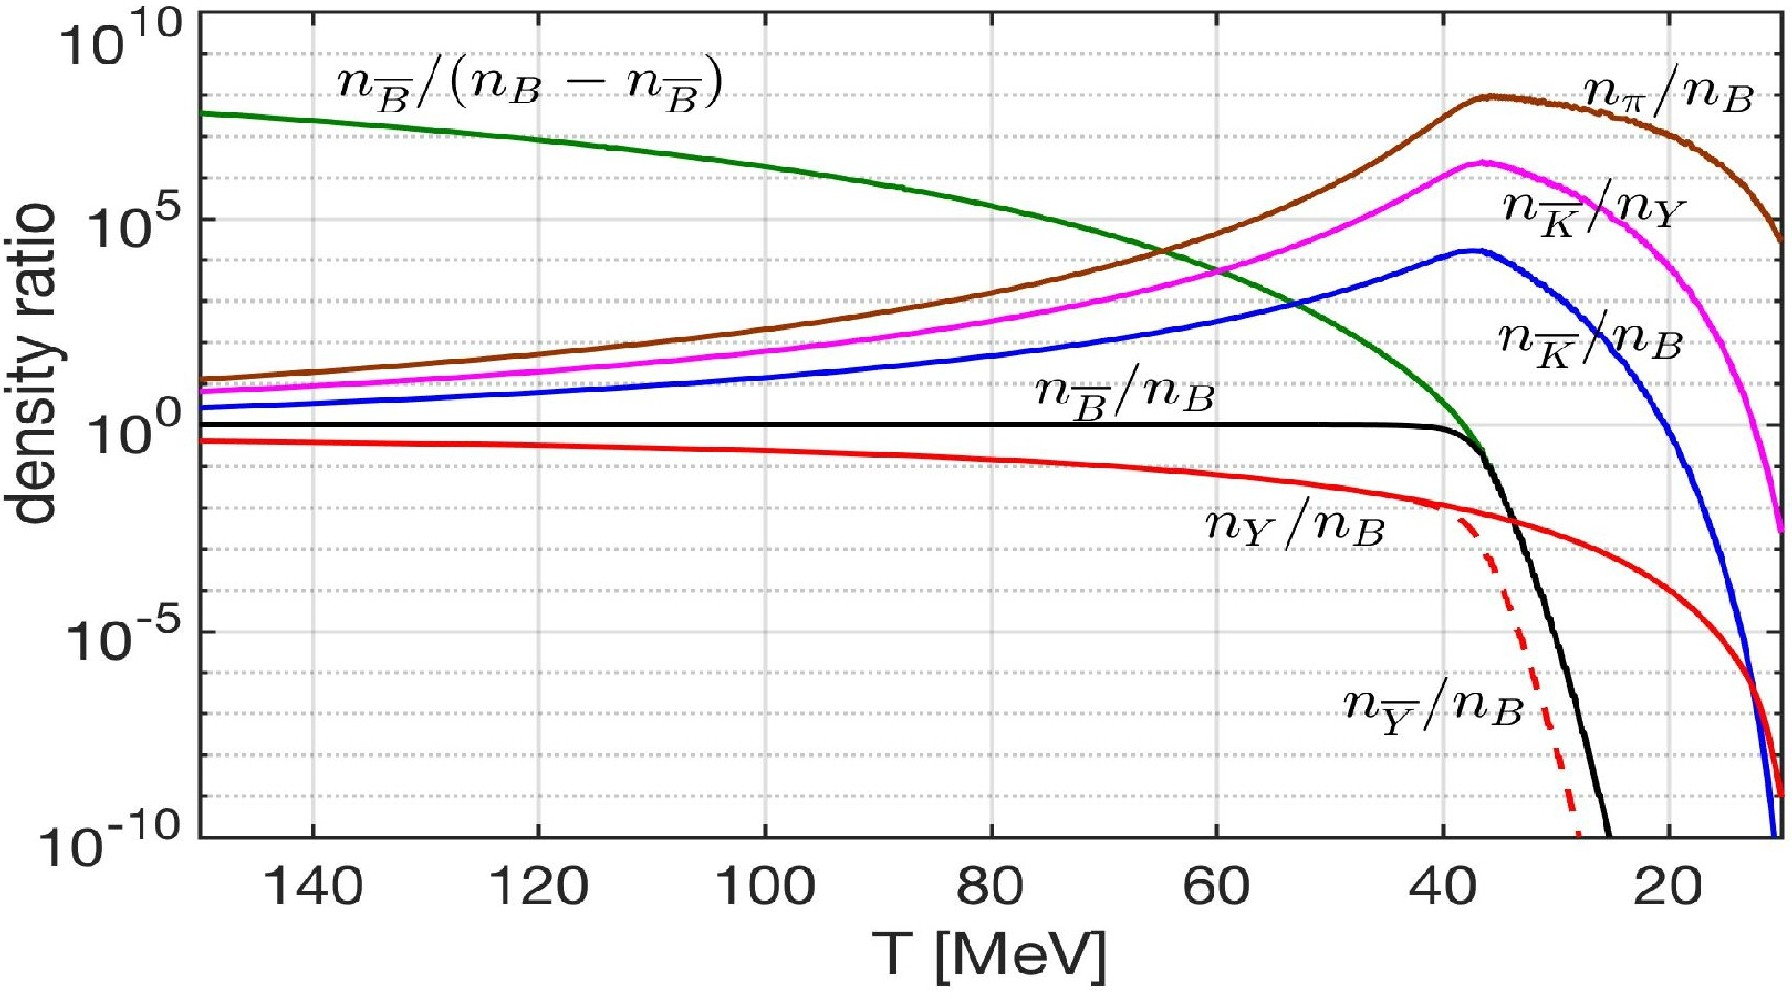
\includegraphics[width=0.9\linewidth]{./plots/Meson_Baryon_density_ratio_C.jpg}}
\caption{Ratios of hadronic particle number densities with baryon $B$ yields as a function of temperature $150\MeV> T>10\MeV$: Pions $\pi$ (brown line), kaons $K( q\bar s)$ (blue), antibaryon $\overline B$ (black), hyperon $Y$ (red) and anti-hyperons $\overline Y$ (dashed red). Also shown $\overline K/Y$(purple). Vertical lines highlight events described in text. \index{strange!hadrons} 
\cccite{Rafelski:2023emw}. \radapt{Yang:2021bko}}
\label{EquilibPartRatiosFig} 
\end{figure}
%%%%%%%%%%%%%%%%%%%%%%%%%%%

%%%%%%%%%%%%%%%%%%%%%%%%%%%%%%%%%
\para{Strange hadron dynamic population}\index{strangeness!dynamic population}
Given the equilibrium abundances of hadrons in the epoch of interest $150\MeV\ge T\ge 10\MeV$, we turn now to study the freeze-out temperature for different particles and strangeness by comparing the relevant reaction rates with each other and with the Hubble expansion rate. We will need to explore a large number of reactions, going well beyond the relative simplicity of the case of QGP phase of matter studied in relativistic heavy ion collisions. We find that strangeness in hadronic particles is kept in equilibrium in the primordial Universe down until $T\approx 13\MeV$. This study addresses non-interacting particles; nuclear interactions can be many times greater compared to this temperature. Thus further exploration of this result seems necessary in the future.

Let us first consider an unstable strange particle $S$ decaying into two particles $1$ and $2$, which themselves have no strangeness content. In a dense and high-temperature plasma with particles $1$ and $2$ in thermal equilibrium, the inverse reaction populates the system with particle $S$. This is written schematically as
\begin{align}
 S\Longleftrightarrow1+2,\qquad \mathrm{Example}: K^0\Longleftrightarrow\pi+\pi\,.
\end{align}
As long as both decay and production reactions are possible, particle $S$ abundance remains in thermal equilibrium; as already discussed this balance between production and decay rates is the `detailed balance'.

Once the primordial Universe expansion rate $1/H$ overwhelms the strongly temperature dependent back-reaction and the back-reaction freeze-out, then the decay $S\rightarrow 1+2$ occurs out of balance and particle $S$ disappears rather rapidly from the inventory. 

Next on our list are the two-on-two strangeness producing and burn-up reactions. These have significantly higher strangeness production reaction thresholds, thus especially near to strangeness decoupling, their influence is negligible. Such reactions are more important near the QGP hadronization temperature $T_H\simeq 150\MeV$. A typical strangeness exchange reaction is $\mathrm{K}+N\leftrightarrow \Lambda+\pi$, (see Chapter 18 in~Ref.\,\cite{Letessier:2002ony}).

In~\rf{Strangeness_map2} we show some reactions relevant to strangeness evolution in the considered Universe evolution epoch $150\MeV\ge T\ge 10\MeV$ and their pertinent reaction strength. Specifically:
\begin{itemize}
\item
We study strange quark abundance in baryons and mesons, considering both open and hidden strangeness (hidden: $s\bar s$-content). Important source reactions are $l^-+l^+\rightarrow\phi$, $\rho+\pi\rightarrow\phi$, $\pi+\pi\rightarrow K_\mathrm{S}$, $\Lambda \leftrightarrow \pi+ N$, and $\mu^\pm+\nu\rightarrow K^\pm$. 
\item
Muons\index{muon} and pions are coupled through electromagnetic reactions $\mu^++\mu^-\leftrightarrow\gamma+\gamma$ and $\pi\leftrightarrow\gamma+\gamma$ to the photon background and retain their chemical equilibrium\index{chemical equilibrium} until the temperature $T =4$\, MeV and $T=5\MeV$, respectively~\cite{Rafelski:2021aey,Kuznetsova:2008jt}. The large $\phi\leftrightarrow K+K$ rate assures $\phi$ and $K$ are in relative chemical equilibrium.
\end{itemize}

%%%%%%%%%%%%%%%%%%%%%%%%%%%%%%%%%%%%%%%
\begin{figure} 
\centerline{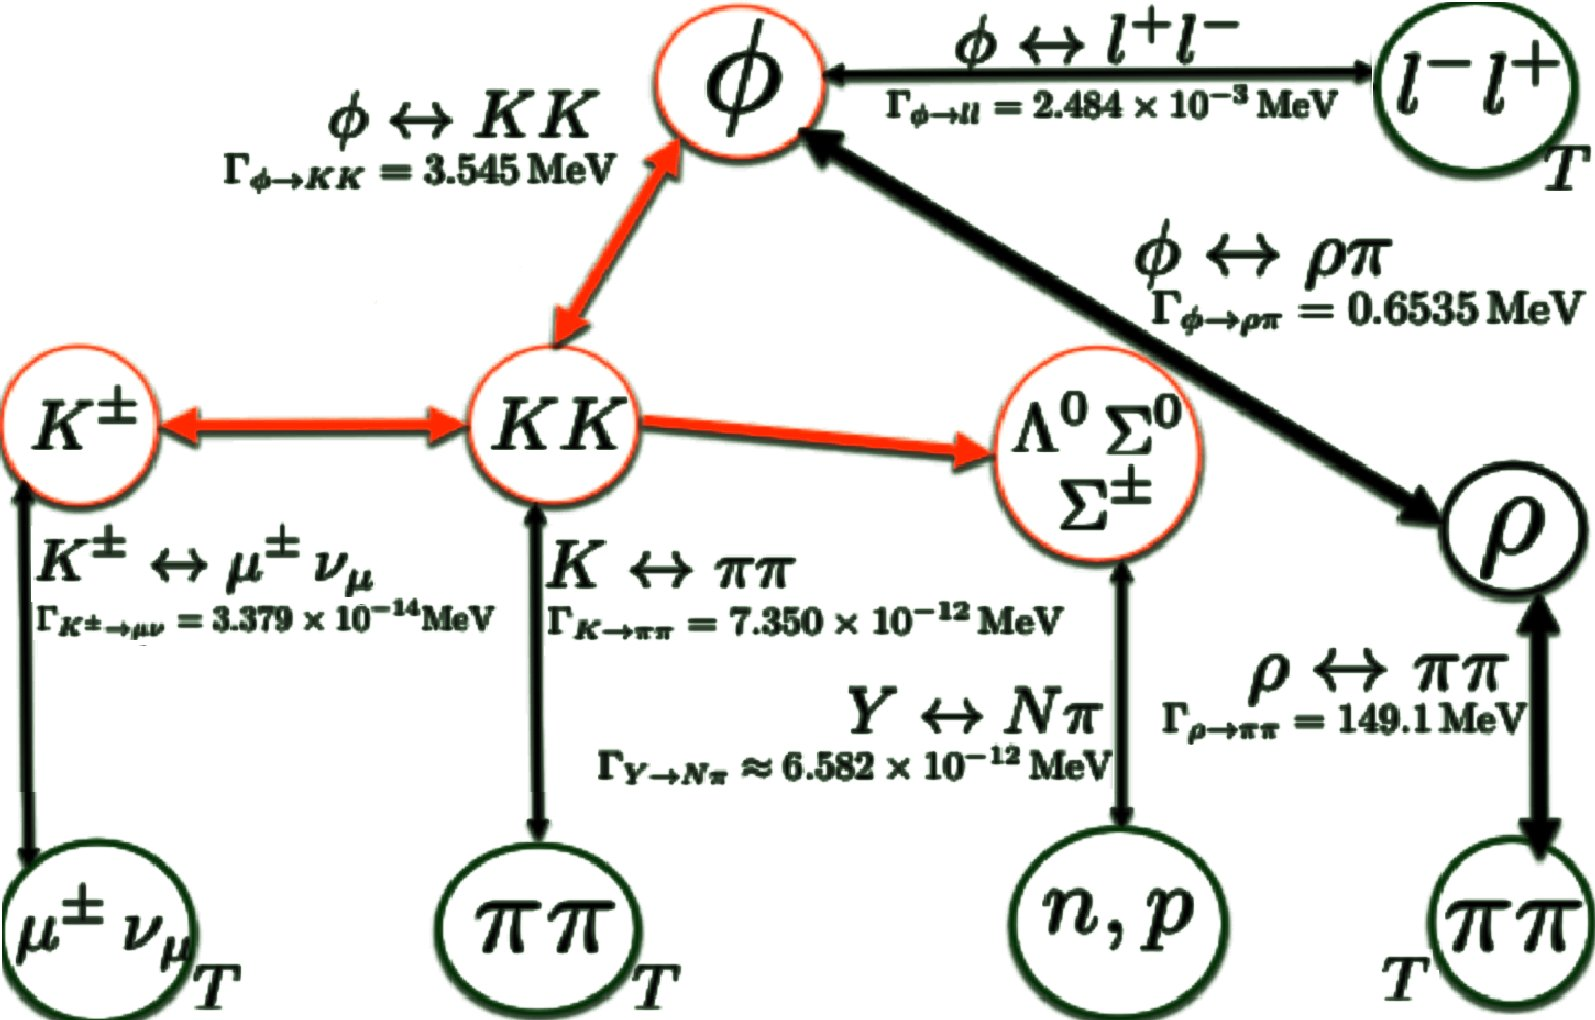
\includegraphics[width=0.85\linewidth]{./plots/Strangeness002_newJ.jpg}}
\caption{The strangeness abundance changing reactions in the primordial Universe. The central circles (red) show strangeness carrying hadronic particles; red thick lines denote effectively instantaneous reactions. Black thick lines show relatively strong hadronic reactions. \cccite{Rafelski:2023emw}. \radapt{Yang:2024ret,Yang:2021bko}}
\label{Strangeness_map2} 
\end{figure}
%%%%%%%%%%%%%%%%%%%%%%%%%%%%%%%%%%%%

In order to determine where exactly strangeness disappears from the Universe inventory, we explore the magnitudes of different rates of production and decay processes in mesons and hyperons and present results in figures. The reaction rates required to describe strangeness time evolution are presented in Ref.~\cite{Rafelski:2020ajx}. 
 
%%%%%%%%%%%%%%%%%%%%%%%%%%%%%%%%%%%%%
\para{Strangeness creation and annihilation rates in mesons}
From~\rf{Strangeness_map2} in the meson domain, the relevant interaction rates competing with Hubble time\index{Hubble!time} are the reactions\index{strangeness!mesons production rate}
\begin{align}
 &\pi+\pi\leftrightarrow K\,,\quad\mu^\pm+\nu\leftrightarrow K^\pm\,,\quad l^++l^-\leftrightarrow\phi\,,\\
 &\rho+\pi\leftrightarrow\phi\,,\quad \pi+\pi\leftrightarrow\rho\,.
\end{align}
The thermal reaction rate per time and volume for two body-to-one particle reactions $1+2\rightarrow 3$ has been presented before~\cite{Koch:1986ud,Kuznetsova:2008jt,Kuznetsova:2010pi}. 

In full kinetic and chemical equilibrium, the reaction rate per time per volume can be written as~\cite{Kuznetsova:2010pi} :\index{inverse decay rate}
\begin{align}
&R_{12\to 3}=\frac{g_3}{(2\pi)^2}\,\frac{m_3}{\tau^0_3}\,\int^\infty_0\frac{p^2_3dp_3}{E_3}\frac{e^{E_3/T}}{e^{E_3/T}\pm1}\Phi(p_3)\;,
\end{align}
where $\tau^0_3$ is the vacuum lifetime of particle $3$. The positive sign `$+$' is for the case when particle $3$ is a boson, and negative sign `$-$' for a fermion. The function $\Phi(p_3)$ for the nonrelativistic limit $m_3\gg p_3,T$ can be written as 
\begin{align}
\Phi(p_3\to0)=2\frac{1}{(e^{E_1/T}\pm1)(e^{E_2/T}\pm1)}.
\end{align}

Considering the Boltzmann\index{Boltzmann!approximation} limit, the thermal reaction rate per unit time and volume becomes
\begin{align}
\label{Thermal_Rate}
R_{12\rightarrow3}=\frac{g_3}{2\pi^2}\left(\frac{T^3}{\tau^0_3}\right)\left(\frac{m_3}{T}\right)^2\,K_1(m_3/T),
\end{align}
where $K_1$ is the modified Bessel\index{Bessel function} functions of integer order `$1$'. 

In order to compare the reaction time with Hubble time $1/H$, it is convenient to define the relaxation time for the process $1+2\rightarrow 3$ as follows:
\begin{align}
\label{Reaction_Time}
\tau_{12\rightarrow 3}\equiv\frac{n^{eq}_{1}}{R_{12\rightarrow n}}\,,\quad
n^{eq}_1=\frac{g_1}{2\pi^2}\int_{m_1}^\infty\!\!\!\!dE\,\frac{E\,\sqrt{E^2-m_1^2}}{\exp{\left(E/T\right)}\pm1}\;, 
\end{align}
where $n^{eq}_1$\,is the thermal equilibrium number density of particle\,$1$ with the `heavy' mass $m_1>T$. Combining \req{Thermal_Rate} with \req{Reaction_Time} we obtain
\begin{align}\label{RelaxationTime}
&\frac{\tau_{12\rightarrow3}}{ \tau^0_3}= 
\frac{2\pi^2 n^{eq}_1/T^3}{g_3(m_3/T)^2\,K_1(m_3/T)}\,, \quad 
n^{eq}_1\simeq g_1\left(\frac{m_1 T}{2\pi}\right)^{3/2}e^{-m_1/T}\,,
\end{align}
where, conveniently, the relaxation time does not depend on the abundant and often relativistic heat bath component $2$, \eg\ $l^\pm,\pi,\nu,\gamma$. The density of heavy particles\,$1$\,and\,$3$ can in general be well approximated using the leading and usually nonrelativistic Boltzmann term as shown above.

In general, the reaction rates for inelastic collision proces  capable of changing particle number, for example $\pi\pi\to K^0$, are suppressed by the factor $\exp{(-m_{K^0}/T)}$. On the other hand, there is no suppression for the elastic momentum and energy exchanging particle collisions in plasma. In general for the case $m\gg T$, the dominant collision term in the relativistic Boltzmann equation is the elastic collision term, keeping all heavy particles in kinetic energy equilibrium with the plasma. This allows us to study the particle abundance in plasma presuming the energy-momentum statistical distribution equilibrium shape exists. This insight was discussed in detail in the preparatory phase of laboratory exploration of hot hadron and quark matter, see~\cite{Koch:1986ud}. 

In order to study the particle abundance in the Universe when $m\gg T$, instead of solving the exact Boltzmann equation, we can separate the fast energy-momentum equilibrating collisions from the slow particle number changing inelastic collisions. This approach makes it possible to explore the rates of inelastic collision and compare the relaxation times of particle production in all relevant reactions with the Universe expansion rate at a fixed temperature which governs the shape of particle distributions.

It is common to refer to particle freeze-out as the epoch where a given type of particle ceases to interact with other particles. In this situation the particle abundance decouples from the cosmic plasma, a chemical nonequilibrium and even complete abundance disappearance of this particle can accompany this; the condition for the given reaction $1+2\rightarrow 3$ to decouple is
\begin{align}
\tau_{12\rightarrow 3}(T_f)=1/H(T_f),
\end{align}
where $T_f$ is the freeze-out temperature.

In the epoch of interest, $150\MeV>T>10\MeV$, the Universe is dominated by radiation and effectively massless matter behaving like radiation. The Hubble parameter can be obtained from the Hubble equation\index{Hubble!equation}
\req{Hubble:eq} and written as~\cite{Kolb:1990vq}
\begin{align}\label{H2g}
H^2=H^2_{rad}\left(1+\frac{\rho_{\pi,\,\mu,\,\rho}}{\rho_\mathrm{rad}}+\frac{\rho_\mathrm{strange}}{\rho_\mathrm{rad}}\right)=\frac{8\pi^3G_\mathrm{N}}{90}g^e_\ast T^4,\qquad H^2_\mathrm{rad}=\frac{8\pi G_\mathrm{N}\,\rho_\mathrm{rad}}{3},
\end{align}
where: $g^e_\ast$ is the total number of effective relativistic `energy' degrees of freedom; $G_\mathrm{N}$ is the Newtonian constant of gravitation; the `radiation' energy density includes $\rho_\mathrm{rad}=\rho_\gamma+\rho_\nu+\rho_{e^\pm}$ for photons, neutrinos, and massless electrons(positrons). The massive-particle correction is $\rho_{\pi,\,\mu,\,\rho}=\rho_\pi+\rho_\mu+\rho_\rho$; and at highest $T$ of interest, also of (minor) relevance, $\rho_\mathrm{strange}=\rho_{K^0}+\rho_{K^\pm}+\rho_{K^\ast}+\rho_{\eta}+\rho_{\eta^\prime}$.
Equating $1/H$ to the computed reaction rate we obtain the freeze-out temperature $T_f$. 

When considering the reaction rates and quoting $T_f$, we must check allowing for a finite reaction time how sudden the freeze-out happens. We refer to this temperature uncertainty as $\Delta T_f$, which by a simple scale consideration can be defined by
\begin{equation}\label{eq:DeltaT}
\Delta T_f\simeq \frac{1}{R(T_f)}\times \frac{dT}{dt}\,. 
\end{equation}
$R$\,[MeV] is the value of reaction rate at freeze-out. The greater is the rate $R_f$ the sharper is the freeze-out, thus smaller $\Delta T_f$.\index{freeze-out!uncertainty}

For the temperature range $50\MeV>T>5\MeV$, we have $10^{-1}<dT/dt<10^{-4}\MeV$/$\mu$s. We estimate the width of the freeze-out temperature interval $\Delta T_f$ using reaction rates for $dt$ as follows
\begin{align}
\frac{1}{\Delta T_f}\equiv \left[\frac{1}{(\Gamma_{12\to3}/H)}\frac{d(\Gamma_{12\to3}/H)}{dT}\right]_{T_f},\quad \Gamma_{12\to3}\equiv\frac{1}{\tau_{12\to3}}.
\end{align}
Using \req{H2g} and \req{RelaxationTime} and considering the temperature range $50\MeV>T>5\MeV$ with $g^e_\ast\approx\mathrm{constant}$ we obtain, using the Boltzmann approximation to describe the massive particles\,$1$\,and\,$3$,
\begin{align}\label{DeltaFreezeout}
 \frac{\Delta T_f}{ T_f} \approx\frac{T_f }{ m_3 - m_1 -2T_f}\,,\quad m_3 - m_1>> T_f\,.
\end{align}
The width of the freeze-out domain is shown in the right column in Table~\ref{FreezeoutTemperature_table}. We see a range of $2$-$10\%$. Therefore it is nearly justified to consider as a decoupling condition in time the value of temperature at which the pertinent rate crosses the Hubble expansion rate, see~\rf{reaction_time_tot}.\index{freeze-out!duration}
 
%%%%%%%%%%%%%%%%%%%%%%%%%%%
\begin{table} 
\centering
\begin{tabular}{c| c| c}
\hline\hline
Reactions &Freeze-out $T_f$\,[MeV] & {Uncertainty $\Delta T_f$\,[MeV]} \\
\hline
$\mu^\pm\nu\rightarrow K^\pm$ & $T_f=33.8\MeV$ & {$3.5$ \,MeV}\\ 
\hline
$e^+e^-\rightarrow \phi$ & $T_f=24.9\MeV$ &{$0.6\MeV$}\\
$\mu^+\mu^-\rightarrow\phi$ & $T_f=23.5\MeV$ &{$0.6\MeV$}\\
\hline
 $\pi\pi\rightarrow K$ & $T_f=19.8\MeV$&{$1.2\MeV$}\\
\hline
$\pi\pi\rightarrow\rho$ & $T_f=12.3\MeV$&{$0.2\MeV$}\\
\hline\hline
\end{tabular}
\caption{Strangeness producing reactions in the primordial Universe, their freeze-out temperature $T_f$; and temperature uncertainty $\Delta T_f$}
\label{FreezeoutTemperature_table} 
\end{table}
%%%%%%%%%%%%%%%%%%%%%%%%%%%%%%%%%%%%%%

%%%%%%%%%%%%%%%%%%%%%%%%%%%%%%%%%%%%%%%%%
\begin{figure}
%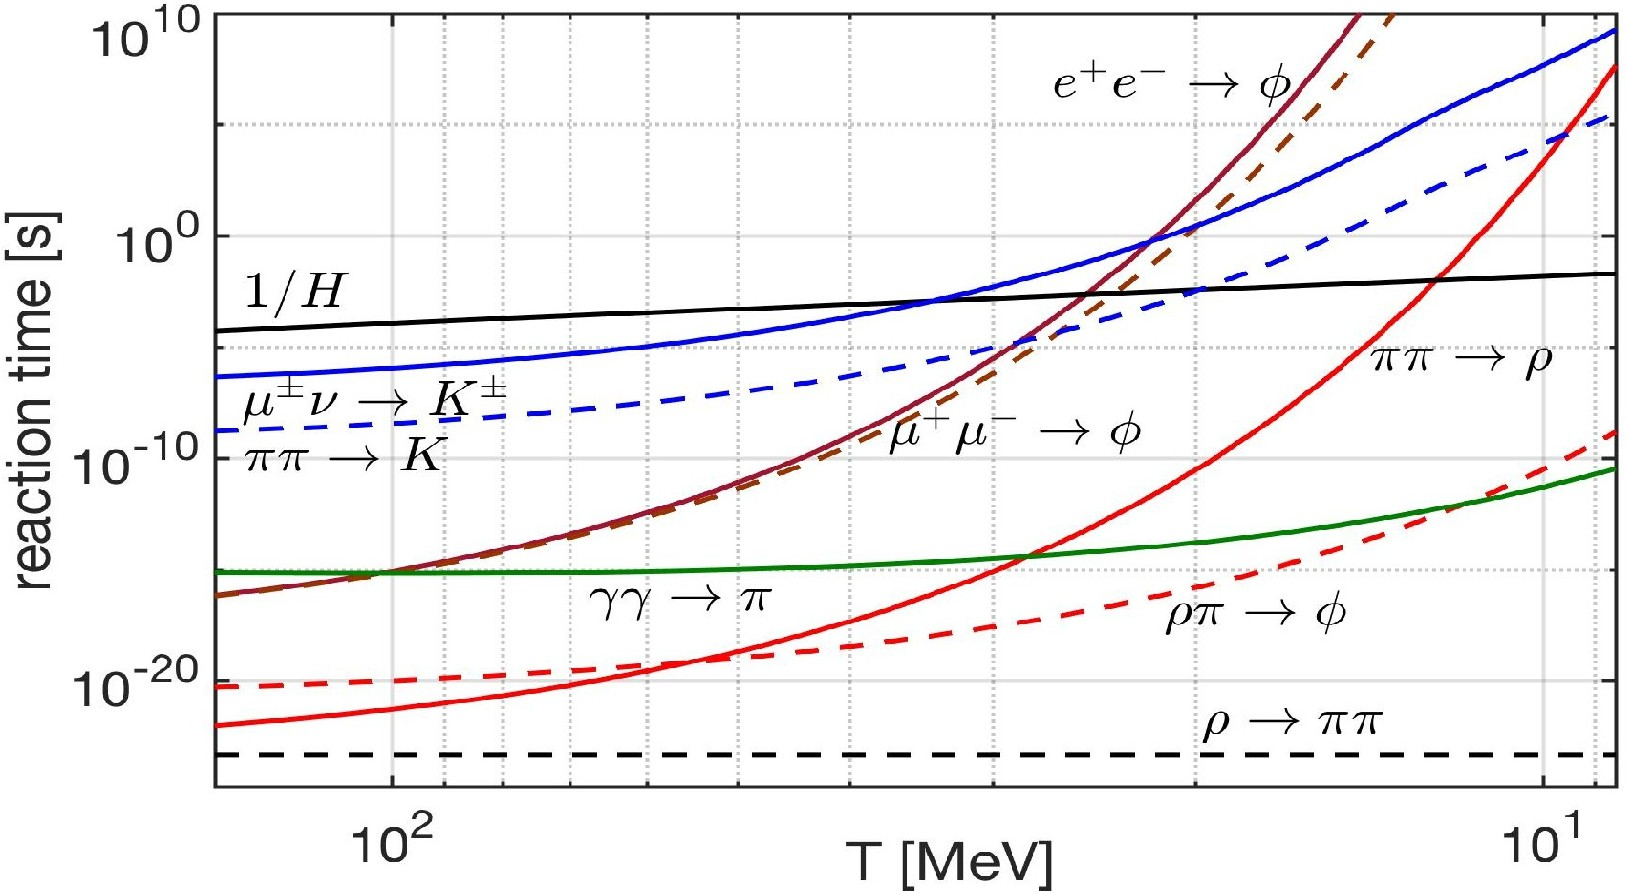
\includegraphics[width=0.95\linewidth]{./plots/Strangeness_Hubble_C.jpg}
\centerline{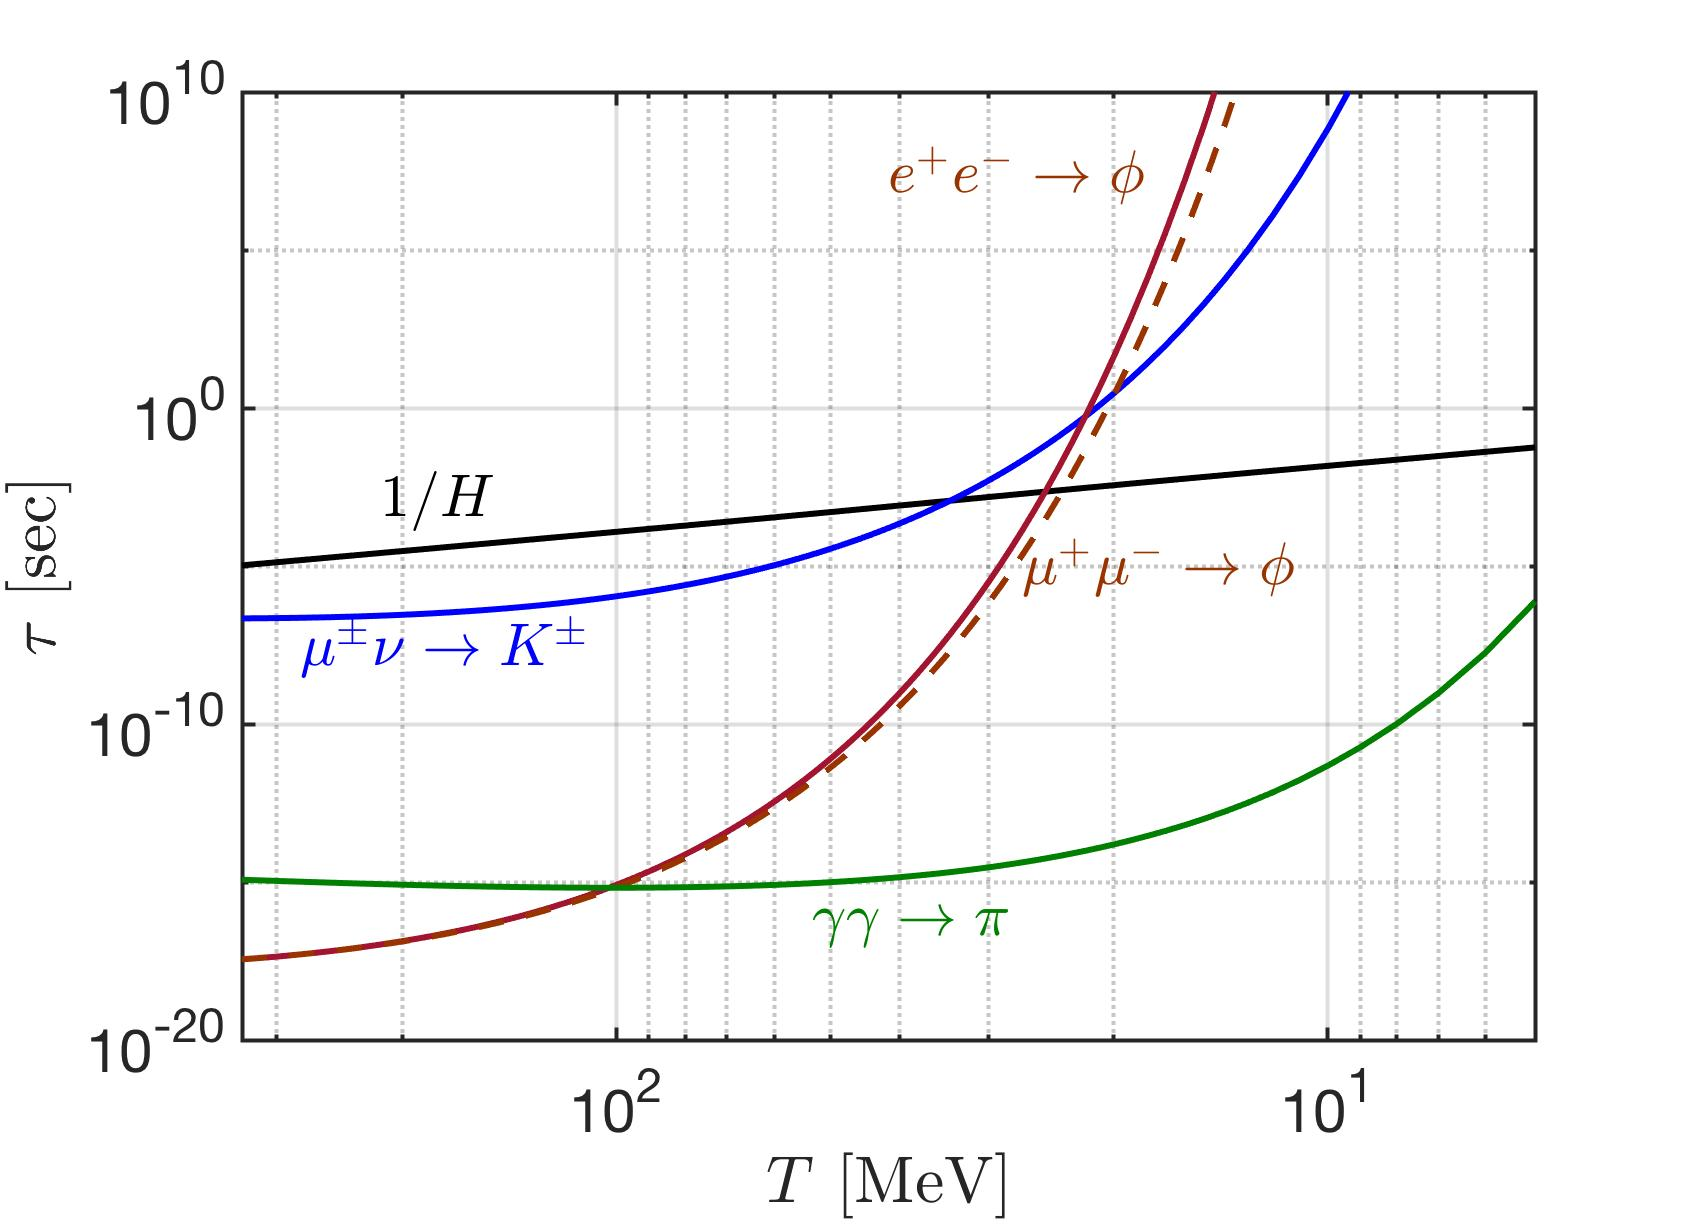
\includegraphics[width=0.9\linewidth]{./plots/Strangeness_Hubble002.jpg}}
\centerline{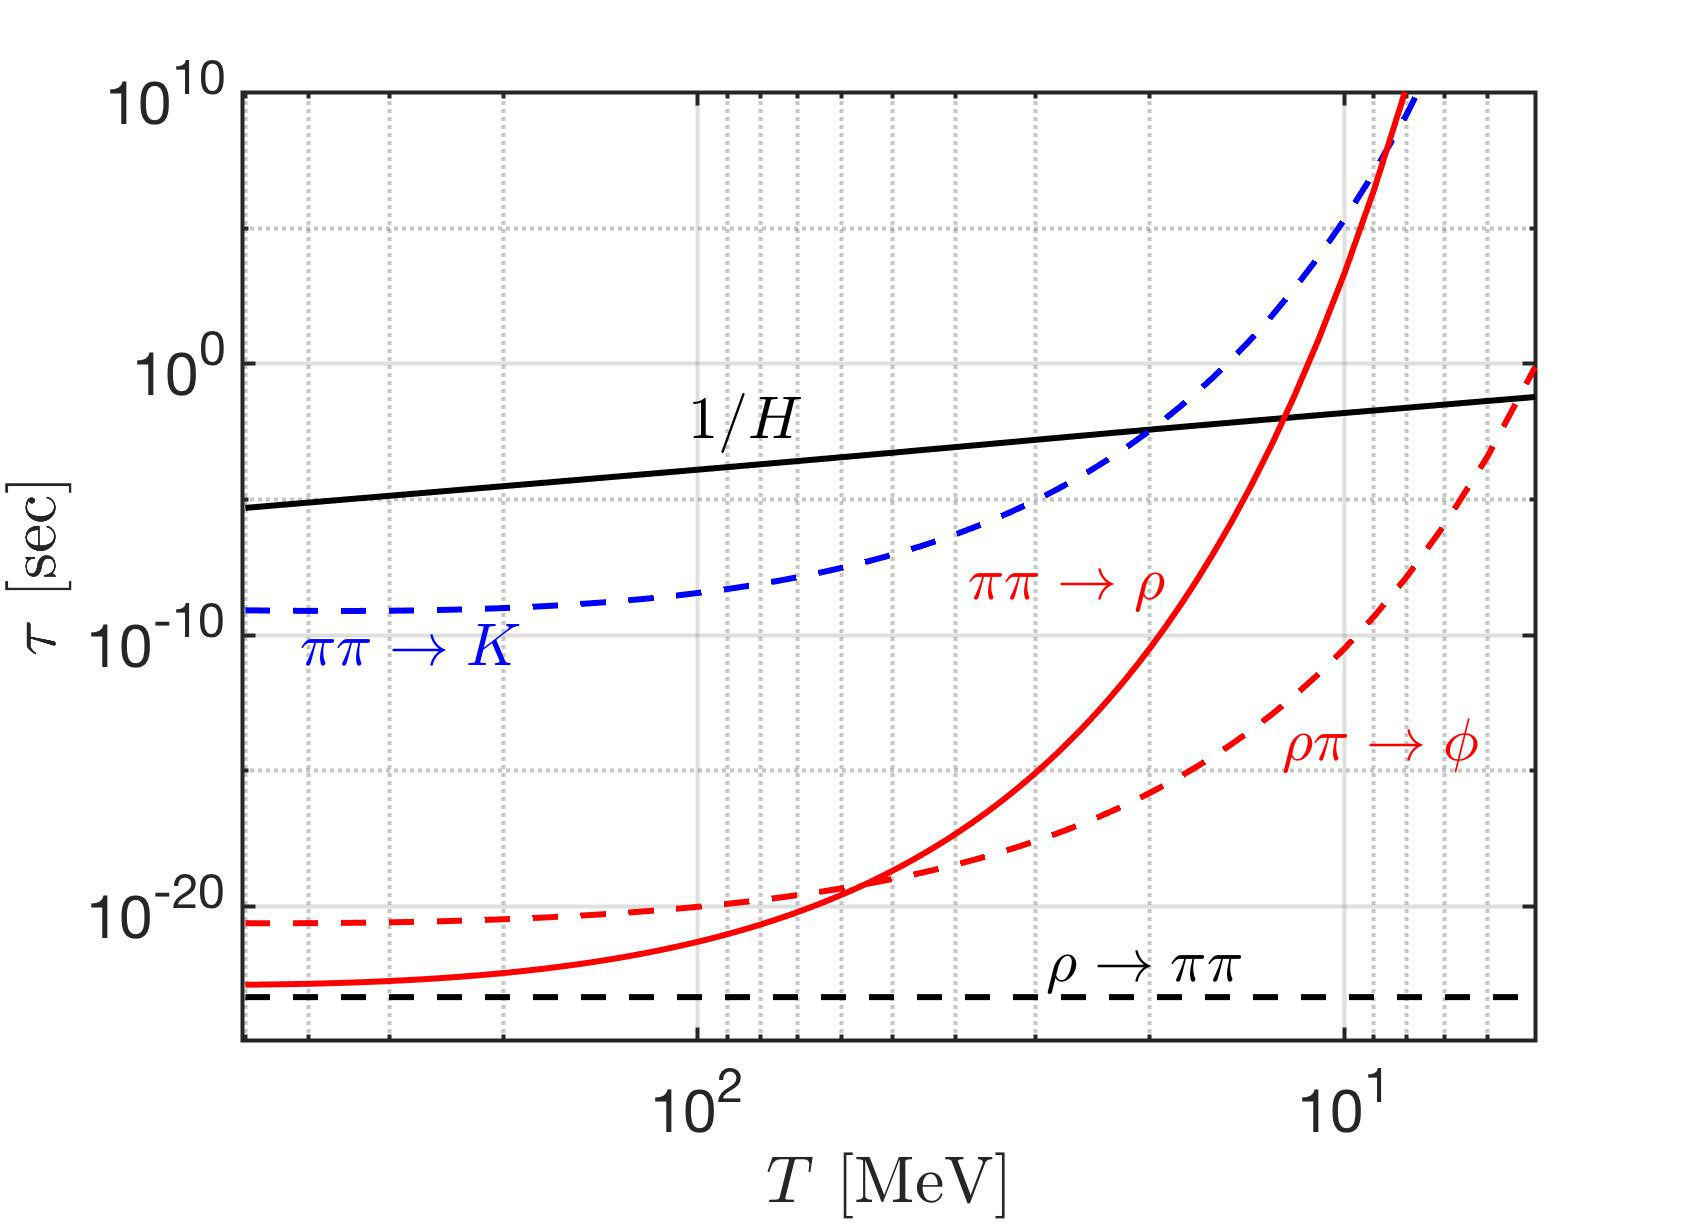
\includegraphics[width=0.9\linewidth]{./plots/Strangeness_Hubble003.jpg}}
\caption{Hadronic relaxation reaction times, see \req{Reaction_Time}, as a function of temperature $T$, are compared to Hubble time $1/H$ (black solid line). At bottom the horizontal black-dashed line is the natural (vacuum) lifespan of $\rho$. \cccite{Rafelski:2023emw}. \radapt{Yang:2024ret,Yang:2021bko}}
\label{reaction_time_tot} 
\end{figure}
%%%%%%%%%%%%%%%%%%%%%%%%

In~\rf{reaction_time_tot} we plot the hadronic reaction relaxation times $\tau_{i}$ in the meson sector as a function of temperature compared to Hubble time $1/H$. We note that the weak interaction reaction $\mu^\pm+\nu_{\mu}\rightarrow K^\pm$ becomes slower compared to the Universe expansion near temperature $T_f^{K^\pm}=33.8\MeV$, signaling the onset of abundance nonequilibrium for $K^\pm$. For $T<T_f^{K^\pm}$, the reactions $\mu^\pm+\nu_{\mu}\rightarrow K^\pm$ decouples from the cosmic plasma; the corresponding detailed balance\index{detailed balance} can be broken and the decay reactions $K^\pm\rightarrow\mu^\pm+\nu_{\mu}$ are acting like a (small) ``hole'' in the strangeness abundance ``pot''. If other strangeness production reactions did not exist, strangeness would disappear as the Universe cools below $T_f^{K^\pm}$. However, there are other reactions: $l^++l^-\leftrightarrow\phi$, $\pi+\pi\leftrightarrow K$, and $\rho+\pi\leftrightarrow\phi$ can still produce the strangeness in cosmic plasma and the rate is very large compared to the weak interaction decay.

In Table~\ref{FreezeoutTemperature_table} we also show the characteristic strangeness reactions and their freeze-out temperatures in the primordial Universe. The intersection of strangeness reaction times with $1/H$ occurs for $l^-+l^+\rightarrow\phi$ at $T_f^\phi=25\sim23\MeV$, and for $\pi+\pi\rightarrow K$ at $T_f^K=19.8\MeV$, for $\pi+\pi\rightarrow\rho$ at $T_f^\rho=12.3\MeV$. The reactions $\gamma+\gamma\rightarrow\pi$ and $\rho+\pi\leftrightarrow\phi$ are faster compared to $1/H$. However, the $\rho\to\pi+\pi$ lifetime (black dashed line in~\rf{reaction_time_tot}) is smaller than the reaction $\rho+\pi\leftrightarrow\phi$; in this case, most the of $\rho$-mesons decays faster, thus are absent and cannot contribute to the strangeness creation in the meson sector. Below the temperature $T<20\MeV$, all the detail balances in the strange meson reactions are broken and the strangeness in the meson sector should disappear rapidly, were it not for the small number of baryons present in the Universe.

%%%%%%%%%%%%%%%%%%%%%%%%%%%%%%%%%%%%%%%%%%%%
\para{Strangeness production and exchange rates involving hyperons}\index{strangeness!hyperons}
In order to understand strangeness in hyperons in the baryonic domain, we now consider the strangeness production reaction $\pi +N\rightarrow K+\Lambda$, the strangeness exchange reaction $\overline{K}+N\rightarrow \Lambda+\pi$; and the strangeness decay $\Lambda\rightarrow N+\pi$. The competition between different strangeness reactions allows strange hyperons and anti-hyperons to influence the dynamic nonequilibrium condition, including development of $\langle s-\bar s\rangle \ne 0$.

To evaluate the reaction rate in two-body reaction $1+2\rightarrow3+4$ in the Boltzmann approximation\index{Boltzmann!approximation} we can use the reaction cross section $\sigma(s)$ and the relation~\cite{Letessier:2002ony}:\index{hyperon!production rate}
\begin{align}
R_{12\rightarrow34}=\frac{g_1g_2}{32\pi^4}\frac{T}{1+I_{12}}\!\!\int^\infty_{s_{th}}\!\!\!\!ds\,\sigma(s)\frac{\lambda_2(s)}{\sqrt{s}}\!K_1\!\!\left({\sqrt{s}}/{T}\right),
\end{align}
where $K_1$ is the Bessel\index{Bessel function} function of order $1$ and the function $\lambda_2(s)$ is defined as
\begin{align}
\lambda_2(s)=\left[s-(m_1+m_2)^2\right]\left[s-(m_1-m_2)^2\right],
\end{align}
with $m_1$ and $m_2$, $g_1$ and $g_2$ as the masses and degeneracy of the initial interacting particle. The factor $1/(1+I_{12})$ is introduced to avoid double counting of indistinguishable pairs of particles; we have $I_{12}=1$ for identical particles and $I_{12}=0$ for others. 

The thermal averaged cross sections for the strangeness production and exchange processes are about $\sigma_{\pi N\rightarrow K\Lambda}\sim0.1\,\mathrm{mb}$ and $\sigma_{\overline{K}N\rightarrow \Lambda\pi}=1\sim3\,\mathrm{mb}$ in the energy range in which we are interested~\cite{Koch:1986ud}. The cross section can be parameterized as follows:\\
1) For the cross section $\sigma_{\overline{K}N\rightarrow \Lambda\pi}$ we use~\cite{Koch:1986ud}
 \begin{align}
 \sigma_{\overline{K}N\rightarrow \Lambda\pi}=\frac{1}{2}\left(\sigma_{K^-p\rightarrow \Lambda\pi^0}+\sigma_{K^-n\rightarrow \Lambda\pi^-}\right)\,.
\end{align}
Here the experimental cross sections can be parameterized as 
\begin{align}
&\sigma_{K^-p\rightarrow \Lambda\pi^0}\!\!=\!\!\left(\begin{array}{l}\!\!1479.53\mathrm{mb}\!\cdot\!\exp{\left(\frac{-3.377\sqrt{s}}{\mathrm{GeV}}\right)},\; \mathrm{for}\,\sqrt{s_m}\!\!<\!\!\sqrt{s}\!<\!3.2\mathrm{GeV} \\ \\0.3\mathrm{mb}\!\cdot\!\exp{\left(\frac{-0.72\sqrt{s}}{\mathrm{GeV}}\right)},\; \mathrm{for}\sqrt{s}>3.2\mathrm{GeV}\end{array}\right.\,,
\\
&\sigma_{K^-n\rightarrow \Lambda\pi^-}\!\!=\!\!1132.27\mathrm{mb}\!\cdot\!\exp{\left(\frac{-3.063\sqrt{s}}{\mathrm{GeV}}\right)},\; \mathrm{for}\sqrt{s}>1.699\mathrm{GeV},
\end{align}
where $\sqrt{s_m}=1.473\GeV$.\\
2) For the cross section $\sigma_{\pi N\rightarrow K\Lambda}$ we use~\cite{Cugnon:1984pm}
\begin{align}
&\sigma_{\pi N\rightarrow K\Lambda}=\frac{1}{4}\times\sigma_{\pi p\rightarrow K^0\Lambda}\,.
\end{align}
The experimental $\sigma_{\pi p\rightarrow K^0\Lambda}$ can be approximated as follows
\begin{align}
\sigma_{\pi p\rightarrow K^0\Lambda}=\left(\begin{array}{l}\frac{0.9\mathrm{mb}\cdot\left(\sqrt{s}-\sqrt{s_0}\right)}{0.091\mathrm{GeV}},\; \mathrm{for} \sqrt{s_0}<\sqrt{s}<1.7\mathrm{GeV} \\ \\ \frac{90\mathrm{MeV\cdot mb}}{\sqrt{s}-1.6\mathrm{GeV}},\; \mathrm{for}\sqrt{s}>1.7\mathrm{GeV},\end{array}\right.
 \end{align}
 with $ \sqrt{s_0}=m_\Lambda+m_K$. 

Given the cross sections, we obtain the thermal reaction rate per volume for strangeness exchange reaction seen in~\rf{Lambda_Rate_volume.fig}. We see that near to $T=20\MeV$, the dominant reactions for the hyperon\index{hyperon} $\Lambda$ production is $\overline{K}+N\leftrightarrow\Lambda+\pi$. At the same time, the $\pi+\pi\to K$ reaction becomes slower than Hubble time and kaon $K$ decay rapidly in the primordial Universe. However, the anti-kaons $\overline K$ produce the hyperon $\Lambda$ because of the strangeness exchange reaction $\overline{K}+N\rightarrow\Lambda+\pi$ in the baryon-dominated Universe. We have strangeness in $\Lambda$ and it disappears from the Universe via the decay $\Lambda\rightarrow N+\pi$. Both strangeness and anti-strangeness disappear because of the $K\rightarrow\pi+\pi$ and $\Lambda\rightarrow N+\pi$, while the strangeness abundance $s = \bar{s}$ in the primordial Universe remains.

%%%%%%%%%%%%%%%%%%%%%%%%%%%%%%%%
\begin{figure} 
\centerline{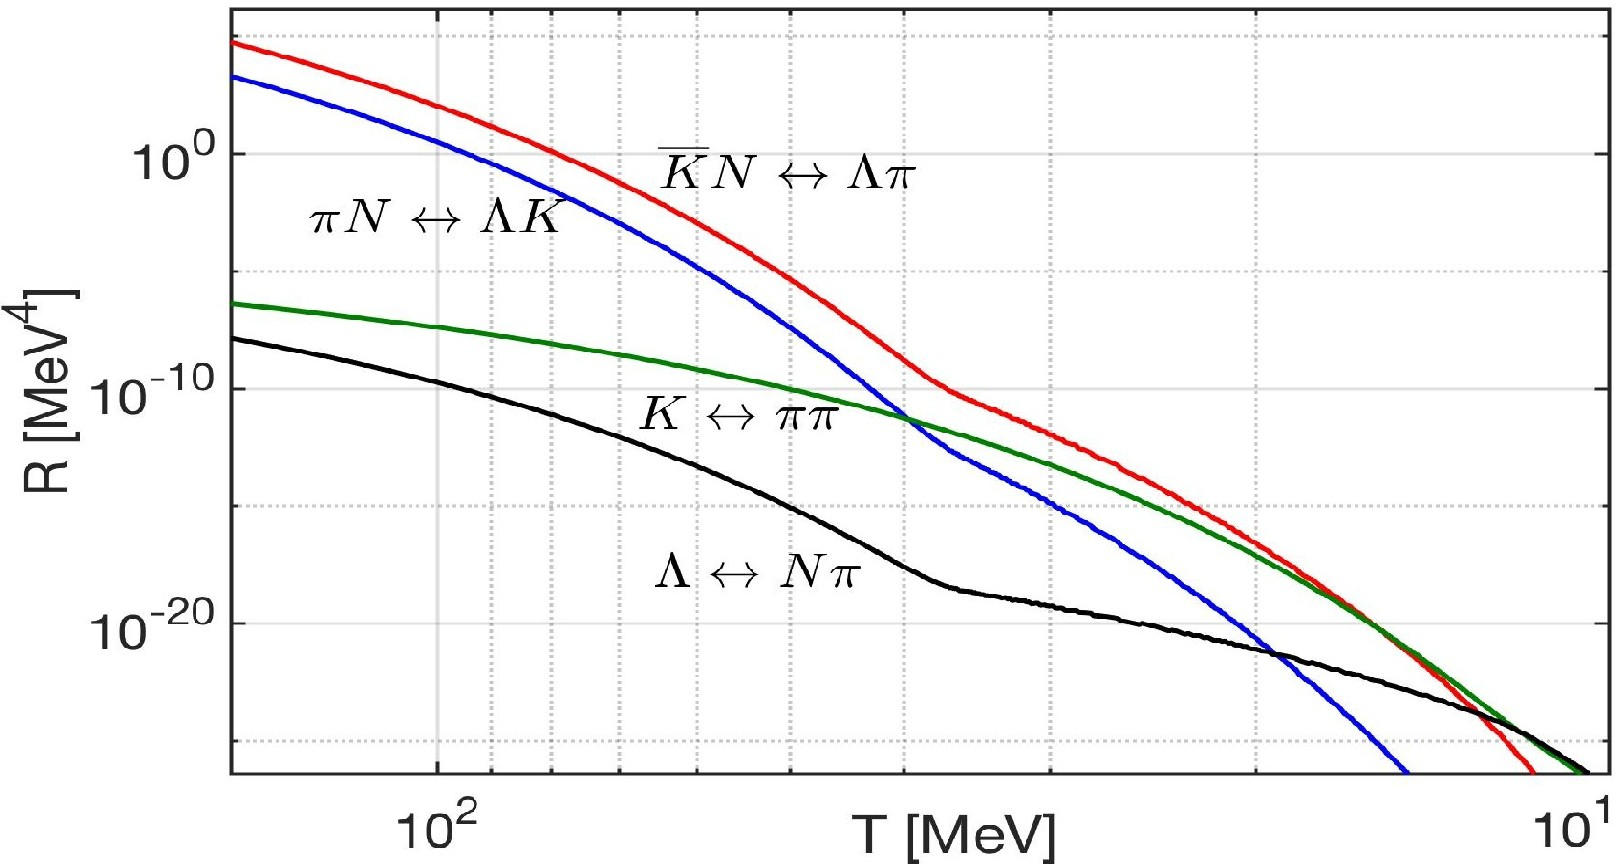
\includegraphics[width=0.9\linewidth]{./plots/NewHyperonRate_C.jpg}}
\caption{Thermal reaction rate $R$ per volume and time for important hadronic strangeness production and exchange processes as a function of temperature $150\MeV> T>10\MeV$ in the primordial Universe. \cccite{Rafelski:2023emw}. \radapt{Yang:2024ret,Yang:2021bko}}
\label{Lambda_Rate_volume.fig} 
\end{figure}
%%%%%%%%%%%%%%%%%%%%%%%%%%%%%%%%%%%%

Near to $T=12.9\MeV$ the reaction $\Lambda+\pi\rightarrow\overline{K}+N$ becomes slower than the strangeness decay $\Lambda\leftrightarrow N+\pi$ and shows that at the low temperature the $\Lambda$ particles are still in equilibrium via the reaction $\Lambda\leftrightarrow N+\pi$ and little strangeness remains in the $\Lambda$. Then strangeness abundance becomes asymmetric $s\gg \bar{s}$, which implies that the assumption for strangeness conservation can only be valid until the temperature $T\sim13\MeV$. Below this temperature a new regime opens up in which the tiny residual strangeness abundance is governed by weak decays with no re-equilibration with mesons. Also, in view of baron asymmetry, $\langle s-\bar s\rangle \ne 0$.

{\color{black}
\para{Strangeness comparison: laboratory with the Universe}\\
In laboratory experiments we study abundance of hadrons present at the instant of chemical freeze-out measuring the value of $T_\mathrm{ch}$, \req{equilibrium}. The dynamic explosive QGP fireball disintegration, often referred to as `sudden hadronization' spans a temperature range which is smaller than the range $155>T_\mathrm{ch}>140\MeV$, the observed production domain which populates particle abundances near to the QGP breakup condition. There is no background of photons, leptons, or neutrinos. 

Said differently, in the laboratory heavy-ion experiments: a) Only strongly interacting degrees of freedom are normally present; b) Particle yields follow from a single chemical freeze-out near to QGP-hadron gas phase cross-over; c) Detailed particle yields allow us to measure the dynamically created chemical potentials; d) An analysis of laboratory experimental data creates a snap-shot image of the abundance freeze-out instant.

In the evolving Universe  we allow for a full adjustment of particle yields to the ambient temperature of the dynamically expanding Universe, and we follow these yields as a function of temperature with chemical potential(s) constrained by the Universe baryon asymmetry. Each particle
has an individual decoupling temperature, with unstable particles usually rapidly disappearing after decoupling, while stable decoupled particles are free-streaming. At low temperature we must consider reactions involving thermal photon, lepton, neutrino background.

A comparison between the early Universe particle inventory and laboratory experiments is implicit in yields seen on the left margin of \rf{EquilibPartRatiosFig}, except for $n_{\overline{B}}/(n_B-n_{\overline{B}})$, which depends on baryon content of the Universe. In this figure the ordinate scale changes by many orders of magnitude since we track the yields over a wide range of temperatures. This prevents us from reading off relevant to heavy-ion collisions results, published in many  other works in past decades.

What this means is that our study of evolving abundances in the Universe is entirely different from laboratory experiments  using same theoretical methods. A detailed comparison between the early Universe particle inventory and laboratory experiments is not insightful.
}